\section{Creating Pictograms}

Issue 135 was to implement a feature allowing users to upload pictures from their device to the backend. The feature description was: "As a \gls{guardian}, I would like a way to add pictograms by choosing an image from my phone gallery so that I can quickly improvise if the system does not have the activity I want."

We expected the feature to require a new screen and a new \gls{bloc} for handling communication with the \gls{api}. We started by designing the view. Since the view should contain as little logic as possible, the \gls{ui} should not have any influence on how we implement the logic. The \gls{ui} also served as a skeleton to implement and test the functionality while developing. We can see the final screen in \autoref{fig:uploadScreen}.

\begin{figure}[!ht]
  \centering
  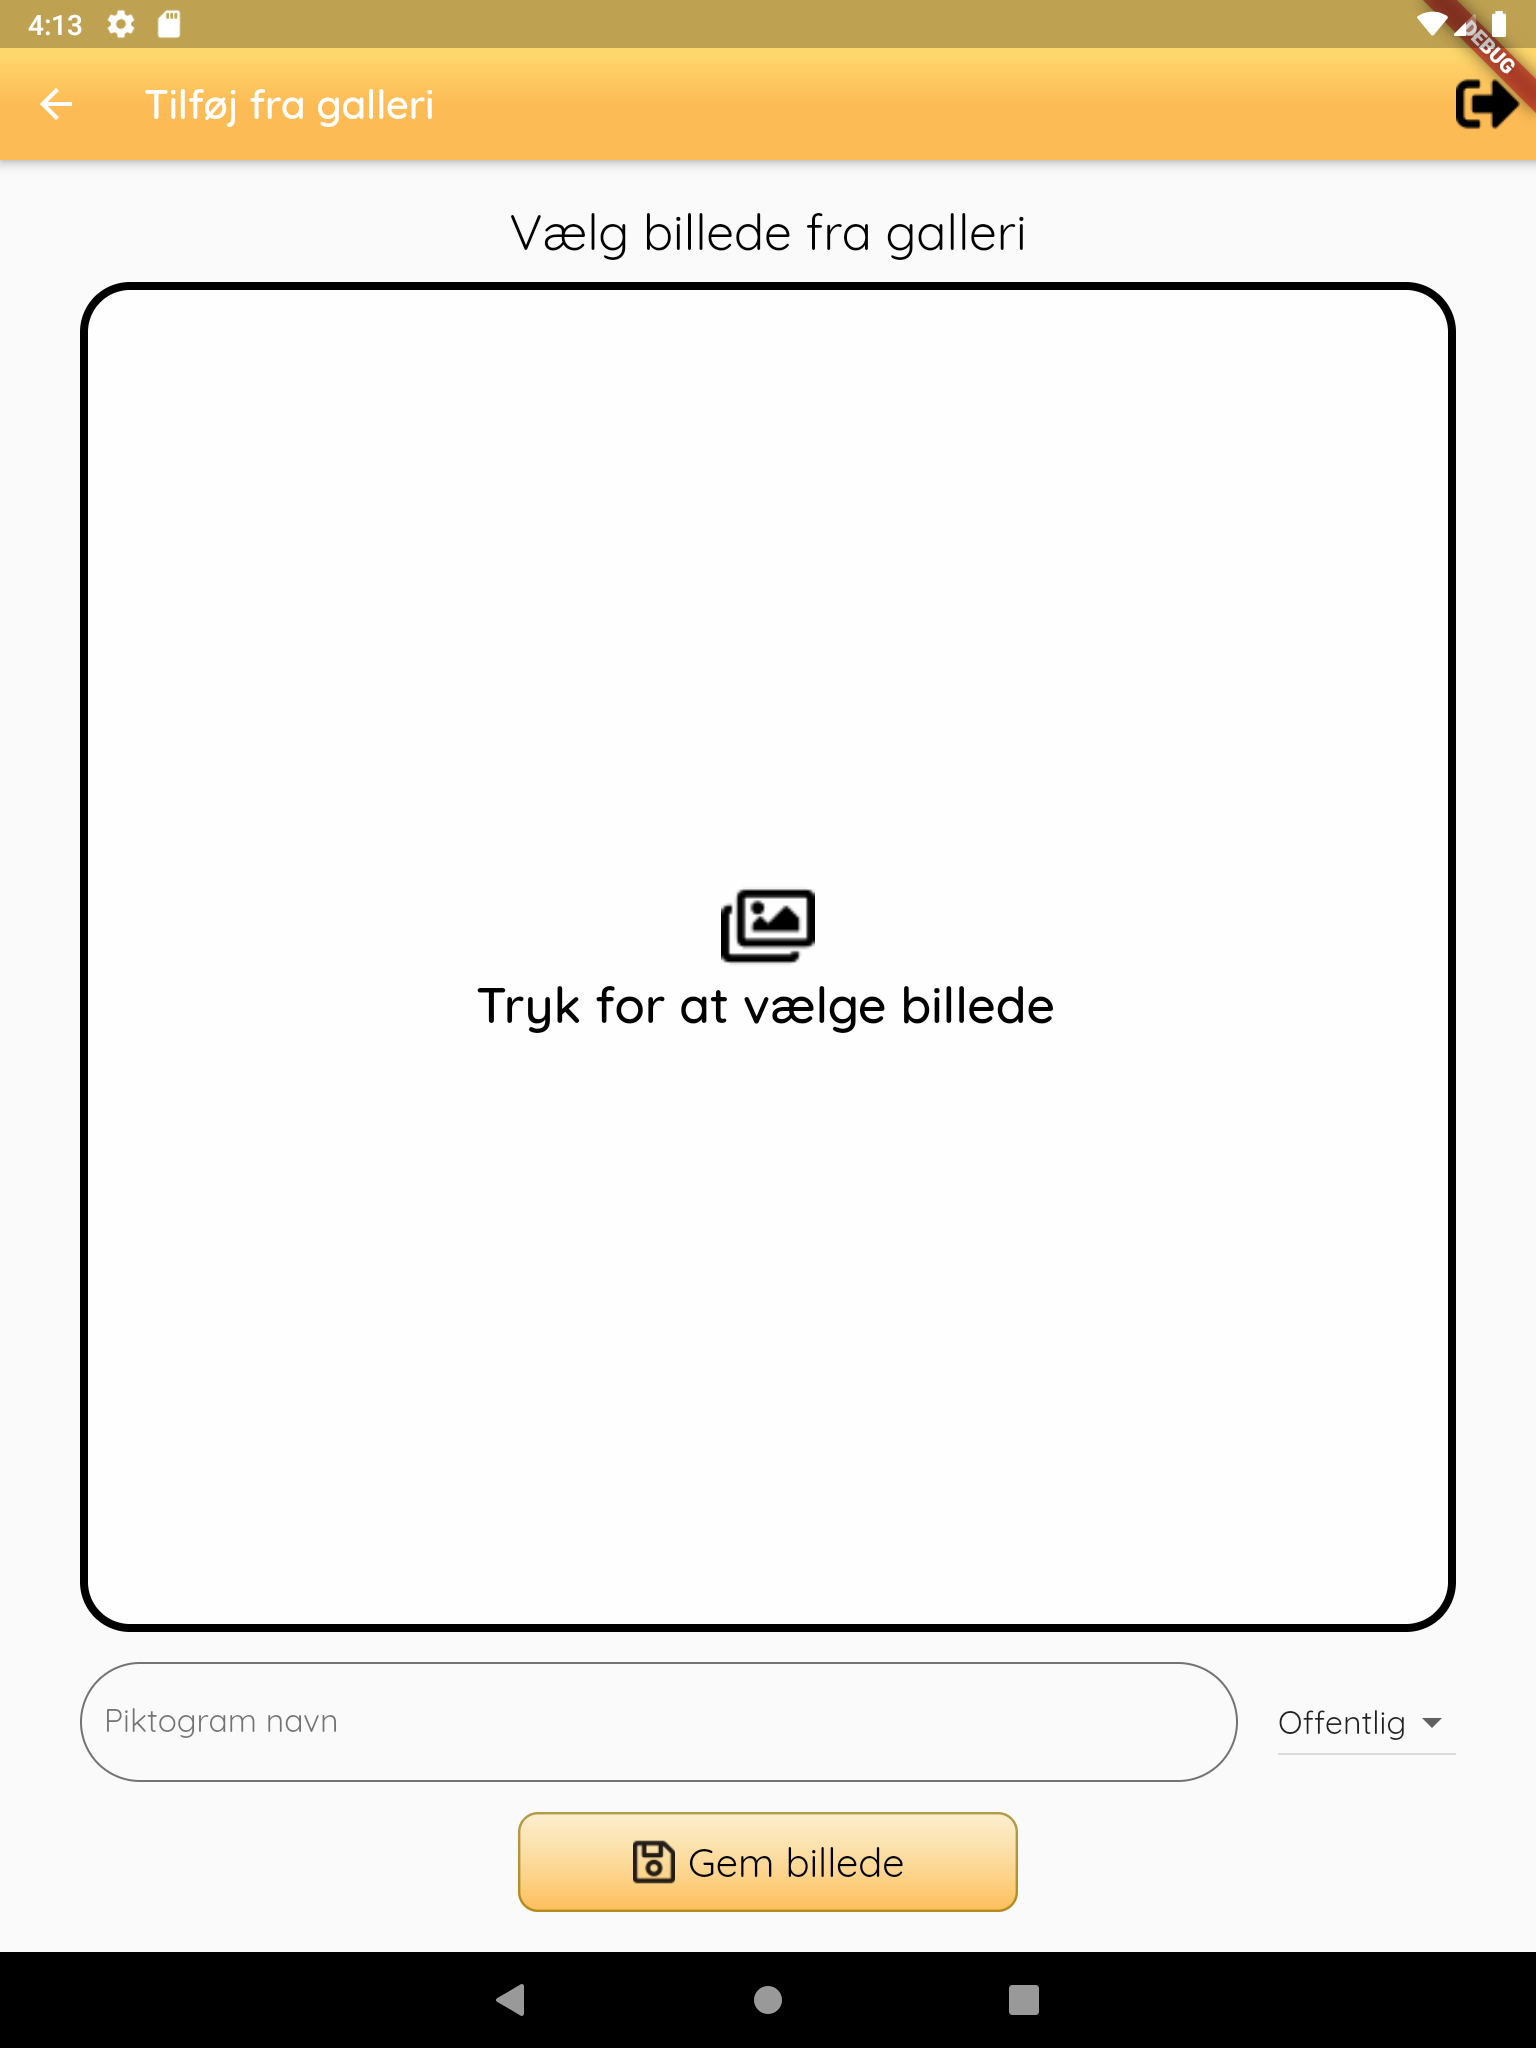
\includegraphics[width=0.7\textwidth]{figures/uploadPictogramScreen.png}
  \caption{Screenshot of the final implementation of the upload image screen}
  \label{fig:uploadScreen}
\end{figure}

We ran into some problems with uploading images as the \gls{fapi} lacked a function to perform the uploading and the backend \gls{api} had some inconsistencies between the specification and implementation of the endpoint for uploading pictograms. 

We mitigated the \gls{fapi} issue without any problems, but the backend \gls{api} had a flaw in its configuration. The endpoint for receiving images filtered the images, only allowing certain types of images, while the later logic expected the image to be in a format already filtered. The expectations of the endpoint were mutually exclusive, which meant that it was not possible to upload images. The endpoint would either reject the request or throw an exception. We aptly fixed this issue, allowing us to send images from the application to the backend.

We also wanted to make the picture uploading process more robust, as currently if the server crashed when receiving the image, it would leave a corrupt file. We added a four-step procedure to combat corruption when creating or editing images. Firstly, we write the byte array to a file with the postfix "\textit{\_temp}". Secondly, we check if there already exists an image for the given pictogram resource, if it does, we postfix that image with "\textit{\_old}", thirdly rename the "\textit{\_temp}" image to the correct filename and lastly delete the "\textit{\_old}" image if it exists.

This four-step procedure ensured that if anything went wrong in the process of the new image, it would always be possible to revert back to the old image.

Testing the implementation on a locally hosted backend server worked perfectly, but since the production environment is a bit different than the local environment, we wanted to assert that it would work on the production environment before committing the solution.

We tested the implementation with the help of the server meta group. They created a copy of the production environment to test on. 

The implementation did not work, and we spent many hours trying to figure out why it worked locally but not in the production environment. We realized that there was an issue between Docker and DotNet Core's \textit{System.IO.File.Move} function. 

We attempted many different workarounds to mitigate the issue between Docker and DotNet Core, but nothing worked. In the end, we concluded that we should either leave this as an open issue for next years students or remove the extra robustness of the upload and write the byte array directly to the file. After consulting with \gls{POT}, they decided that we should implement the feature without the additional robustness.

When debugging the uploading issue, we identified and promptly fixed issues in the system. We discovered that all the deployed backend environments (production, development, and testing) used the same file location for pictograms, which meant that when testing the file upload we affected the data for production and development. The server group fixed this issue and ensured that every deployed backend has its designated file location for pictograms. Another discovery was that the production and development deployments used the same database, which we also fixed.

In the end, the feature was implemented successfully, with the compromise that if something goes wrong in the upload process, a corrupt file can be introduced into the system.
